	\documentclass[twoside]{article}
\usepackage{../../estilo-ejercicios}
\renewcommand{\baselinestretch}{1,4}
%--------------------------------------------------------
\begin{document}

\title{Éléments de Géométrie Algébrique, Remarque 2.3.6}
\author{Javier Aguilar Martín}
\maketitle

%\varprojlim
%\varinjlim
\section{Pasos previos}

\begin{defi}[EGA, 1.1.9]
En una categoría $\CC$, dado un conjunto parcialmente ordenado $I$, se define un \emph{sistema proyectivo} como una familia $(A_\alpha)_{\alpha\in I}$ de objetos de $\CC$ y para cada par $(\alpha,\beta)$ tal que $\alpha\leq\beta$ un morfismo $u_{\alpha\beta}:A_\alpha\to A_\beta$ cumpliendo $u_{\alpha\gamma}=u_{\alpha\beta}\circ u_{\beta\gamma}$ para $\alpha\leq\beta\leq\gamma$. Un \emph{límite proyectivo} de un sistema proyectivo está formado por un objeto $B\in\CC$ (denotado $\varprojlim A_\alpha$), y para cada $\alpha\in I$, un morfismo $u_\alpha:B\to A_\alpha$ tales que: 
\begin{enumerate}
\item $u_\alpha=u_{\alpha\beta}u_{\beta}$ para $\alpha\leq\beta$;
\item para todo objeto $X$ de $C$ y toda familia $(v_\alpha)_{\alpha\in I}$ de morfismos $v_\alpha:X\to A_{\alpha}$ verificando $v_\alpha=u_{\alpha\beta}v_{\beta}$ para $\alpha\leq\beta$, existe un único morfismo $v:X\to B$ (denotado $\varprojlim v_\alpha$) tal que $v_\alpha=u_\alpha v$ para todo $\alpha\in I$
\[
\begin{tikzcd}
& & & & X\arrow[dlll, bend left=-20, "v_\alpha"]\arrow[dll, bend left=-15, "v_\beta"]\arrow[dl, bend left=-10, "v_\gamma"]\arrow[dd, dashed, bend left, "\varprojlim v_\alpha"]\\
\cdots\arrow[r] &A_\alpha \arrow[r, "u_{\alpha\beta}"] & A_\beta \arrow[r, "u_{\beta\gamma}"] & A_\gamma\arrow[r] &\cdots\\
&  & & & \varprojlim A_\alpha\arrow[ulll, bend left=20, "u_\alpha"]\arrow[ull, bend left=15, "u_\beta"]\arrow[ul, bend left=10, "u_\gamma"]
\end{tikzcd}
\]
\end{enumerate}
Decimos que $\CC$ \emph{admite límites proyectivos} si siempre existen límites proyectivos de sistemas proyectivos en $\CC$. 
\end{defi}

%EN TOP ES INTERSECCIÓN CON TOPOLOGÍA INICIAL (LA QUE CON MENOS ABIERTOS HACE CONTINUAS A TODAS LAS FLECHAS AL SISTEMA PROJECTIVO) POR EL EJERCICIO 1.12 DE HARTSHORNE EL LÍMITE INVERSO DE HACES ES HAZ
EL LÍMITE INVERSO EN ESPACIOS TOPOLÓGICOS POR SI ME HACE FALTA, DE TODOS MODOS EN SET SEGURAMENTE SÍ ME HAGA FALTA\url{https://math.stackexchange.com/questions/711334/inverse-limit-of-an-inverse-system-of-topological-spaces}

\begin{prop}[EGA, 3.2.6]\label{limite}
Sea $\CC$ una categoría que admite límites proyectivos y $X$ un espacio topológico. La categoría de haces sobre $X$ con valores en $C$ admite límites proyectivos. 
\end{prop}
\begin{dem}
PRUEBA DEL 1.12 DE HARTSHORNE PERO GENERALIZADA
\end{dem}

\begin{ej}[$\mathrm{Set}$ admite límites proyectivos]\label{set}
CONSTRUIR EL LÍMITE PROYECTIVO Y PROBAR QUE LO ES
\end{ej}

\begin{remarque}{4.5.6}
Llamamos \emph{prehaz} sobre una categoría $\CC$ a un functor $F:\CC^{op}\to\mathrm{Set}$. Denotamos por $\mathrm{Top}_{Ring}|_S$ a la categoría de espacios anillados sobre un espacio anillado fijo $S$, esto es la categoría cuyos objetos son morfismos en $\mathrm{Top}_{Ring}$ de la forma $X\to S$ (a los que llamamos $S$-espacios) y los morfismos son morfismos $X\to Y$ (llamados $S$-morfismos) en $\mathrm{Top}_{Ring}$ que hacen conmutativo el diagrama
\[
\begin{tikzcd}
X\arrow[r]\arrow[dr] & Y\arrow[d]\\
 & S
\end{tikzcd}
\]

Un prehaz 
\begin{equation}\label{representable}
F:(\mathrm{Top}_{Ring}|_S)^{op}\to\mathrm{Set}
\end{equation}
 nos da para todo $S$-espacio $X$ un prehaz de conjuntos $U\to F(U)$ sobre $X$, ya que los abiertos de $X$ tienen una estructura inducida de $S$ espacio. Cuando para todo $S$-spacio $X$ este prehaz es un haz, decimos que $F$ es un \emph{haz sobre la categoría} $\mathrm{Top}_{Ring}|_S$, noción que se puede generalizar a cualquier categoría usando la topología de Grothendieck de una categoría, aunque no la necesitaremos para nuestros propósitos. Estos functores forman una subcategoría plena de $\Hom((\mathrm{Top}_{Ring}|_S)^{op},\mathrm{Set})$ denotada $\Sh_{\mathrm{Top}_{Ring}|_S}$. Si añadimos a esto la proposición \ref{limite} y el ejemplo \ref{set}, resulta que $\Sh_{\mathrm{Top}_{Ring}|_S}$ admite límites proyectivos de sistemas proyectivos de functores que son haces sobre un mismo espacio $X$ NO SÉ SI ME HARÁ FALTA QUE EXISTAN PARA ESPACIOS DISTINTOS. %COGE COMO ESPACIO EL LÍMITE INVERSO COMO DIGO ARRIBA Y EL HAZ TAMBIÉN LÍMITE INVERSO

%RECUERDA LA DEFINICIÓN DE FUNCTOR REPRESENTABLE, EN ESTE CASO EL FUNCTOR ES REPRESENTABLE PORQUE DE HECHO ES UN ELEMENTO DE HOM(A,-)

Un functor representable como \ref{representable} es siempre un haz: es claro que en efecto el prehaz $U\mapsto\Hom_S(U,Z)$ sobre un espacio anillado $X$ es un haz, ya que para todo recubrimiento abierto $(U_\alpha)$ de un abierto $U\subseteq X$, dar un $S$-morfismo de $U\to Z$ equivale a dar una familia de $S$-morfismos $f_\alpha:U_\alpha\to Z$ tales que para toda pareja de índices $(\alpha,\beta)$ las restricciones de $f_\alpha$ y $f_\beta$ a $U_\alpha\cap U_\beta$ coincidan.

Por el lema de Yoneda podemos decir además que tenemos un functor plenamente fiel $Z\to h_Z$ de la categoría $\mathrm{Top}_{Ring}|_S$ a la categoría $\Sh_{\mathrm{Top}_{Ring}|_S}$, que nos permite identificar la primera categoría con una subcategoría plena de la segunda %COMO UN FUNCTOR REPRESENTABLE ES SIEMPRE UN HAZ, LA IMAGEN ESENCIAL DE FUNCTOR H_Z CAE EN SH


\end{remarque}

\begin{remarque}{4.5.7}
ME HACE FALTA PARA DECIR QUE ME LA PUEDO LLEVAR A LOCALMENTE ANILLADOS
\end{remarque}


\section{Remarque 3.2.6}

TENGO QUE COMPROBAR QUE LAS OBSERVACIONES DE ANTES VALEN PARA ESQUEMAS 
%\begin{solucion}
%
%\end{solucion}
%
%\newpage
%
%
%\begin{ejercicio}{1.2}
%
%\end{ejercicio}
%\begin{solucion}
%
%\end{solucion}
%
%\newpage
%DECIRLE QUE QUIERO HACER EL 2.16


%\begin{ejercicio}{3.1}
%Probar que un morfismo $f:X\to Y$ es localmente de tipo finito si y solo si para \emph{todo} abierto afín $V=\spec(B)$ de $Y$, $f^{-1}(V)$ puede ser cubierto por abiertos afines $U_j=\spec(A_j)$, donde cada $A_j$ es una $B$-álgebra finitamente generada. 
%\end{ejercicio}
%\begin{solucion}
%%Una de las implicaciones es trivial, así que supongamos que $f:X\to Y$ es localmente de tipo finito. Sea $V=\spec(B)$ un abierto afín de $Y$ y consideremos $f^{-1}(V)$. Por ser $f$ localmente de tipo finito, podemos recubrir $Y$ con abiertos afines $V_i=\spec(B_i)$ de modo que $f^{-1}(V_i)$ está cubierto por abiertos afines $U_{ij}=\spec(A_{ij})$, donde cada $A_{ij}$ es na $B_i$-álgebra finitamente generada. %Esto nos da un recubrimiento de $f^{-1}(V)$ por abiertos de $X$, ya que $f^{-1}(V)=f^{-1}(V\cap \bigcup V_i)=\bigcup(f^{-1}(V)\cap f^{-1}(V_i))$, pero estos abiertos no tienen por qué ser afines. 
%%
%%Observemos que para $\p\in B_i$, $f^{-1}(\spec((B_i)_\p))$ está cubierto por los $f^{-1}(\spec((A_{ij})_{\p^e})$, donde el ideal $\p^e$ es el extendido de $\p$ por la aplicación del álgebra $B_i\to A_{ij}$: si $f(x)\in\spec((B_i)_{\p})$, entonces $f(x)$ es un primo de $B_i$ que no contiene a $\p$, por lo que 
%
%%\url{https://math.stackexchange.com/questions/384137/intersection-of-open-affines-can-be-covered-by-open-sets-distinguished-in-both}
%%\url{https://math.arizona.edu/~cais/CourseNotes/AlgGeom04/Hartshorne_Solutions.pdf}
%%\url{https://math.stackexchange.com/questions/2588088/prime-ideals-of-a-localization}
%%
%%
%%NUEVA IDEA
%%
%%
%%\url{http://mathbabysteps.blogspot.com/2016/12/affine-communication-lemma.html}
%%\url{https://math.stackexchange.com/questions/803636/question-on-morphism-locally-of-finite-type}
%
%Una de las implicaciones es trivial, así que supongamos que $f:X\to Y$ es localmente de tipo finito. Sea $V=\spec(B)$ un abierto afín de $Y$. Del recubrimiento afín $\{V_i=\spec(B_i)\}_{i\in I}$ de $Y$ que nos da que $f$ sea localmente de tipo finito obtenemos un recubrimiento afín de $V$, pero $V\cap V_i$ no será en general afín, así que necesitamos el siguiente lema:
%
%\begin{lemma}
%Sean $U=\spec(A)$ y $V=\spec(B)$ subesquemas afines abiertos de un esquema $X$. Entonces $\spec(A)\cap\spec(B)$ puede ser recubierto por abiertos $W_i$ que son subesquemas abiertos básicos tanto de $\spec(A)$ como de $\spec(B)$.
%\end{lemma}
%\begin{proof}
%Hacemos primero la siguiente observación: dado un abierto $U$ y $g\in\OO_X(U)$ y $V\subseteq U$, denotamos $U_g=\{x\in U\mid g_x\notin \mm_x\}$ donde $\mm_x$ es el ideal maximal de $\OO_x$, entonces $U_g\cap V=V_{g|_V}$. 
%
%Sea $p\in\spec(A)\cap\spec(B)$. Afirmamos que existe un subesquema abierto básico tanto de $\spec(A)$ como de $\spec(B)$ conteniendo a $x$. Sea $\spec(A)\supseteq\spec(A_f)\ni p$ y sea $\spec(A_f)\supseteq\spec(B_g)\ni p$ tal como se observa en la figura.
%\begin{figure}[h!]
%\centering
%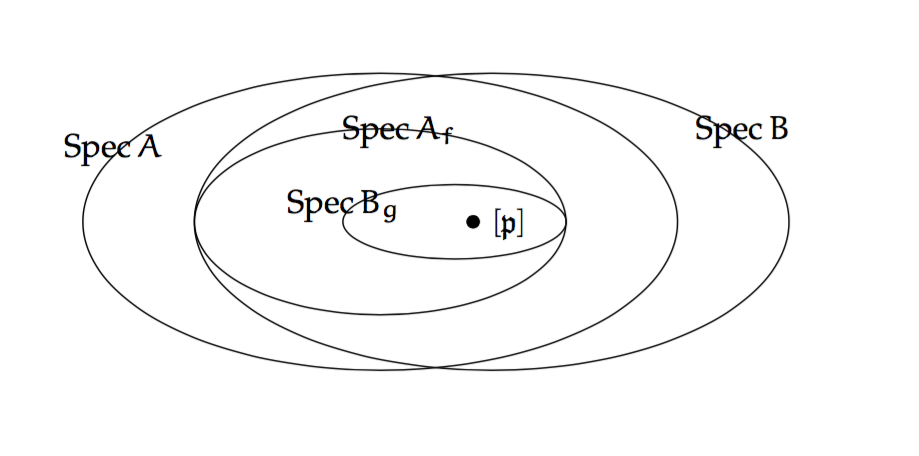
\includegraphics[scale=0.22]{3-1}
%\end{figure}
%
% Estas inclusiones y el hecho de que $\spec(A_f)$ es básico en $\spec(A)$ y $\spec(B_g)$ es básico en $\spec(B)$ nos lo da el ejercicio 2.1. Vamos a probar que $\spec(B_g)$ también es básico en $\spec(A)$. Tenemos que $g\in\Gamma(\spec(B),\OO_X)$ se restringe a $g'\in\Gamma(\spec(A_f),\OO_X)=A_f$. Por la observación del principio de la demostración tenemos que $\spec(B_g)=\spec(A_f)_{g'}$. Si $g'=g''/f^n$ con $g''\in A$, tal como se hizo en el apartado (a) del ejercicio 2.16 se prueba que además $\spec(A_f)_{g'}=\{x\in\spec(A)\mid (f^ng'')_x=g'_x\notin \mm_x\}=D(g')$, con lo que hemos probado el resultado. 
%
%
%
%\end{proof}
%Ahora podemos cubrir $V$ con subesquemas afines que son básicos tanto en $V$ como en $V_i$, y tomando preimágenes recubrimos $f^{-1}(V)$ (aunque cada preimagen no tiene por qué ser afín). Sea $V'$ unos de esos subesquemas afines, digamos $D(g)=V'= D(g_i)$ con $g\in B$ y $g_i\in B_i$. Podemos cubrir $f^{-1}(V')$ por subesquemas affines abiertos que son abiertos básicos para unos ciertos abiertos afines $U_{ij}=\spec(A_{ij})$ de $X$ (los que nos da que $f$ sea localmente de tipo finito). Sea $U'$ uno de esos abiertos básicos, digamos $U'=D(f_{ij})$ para $f_{ij}\in A_{ij}$. 
%
%Ahora, $f|_{U_{ij}}:U_{ij}\to V_i$ está inducida por un homomorfimos de anillos $\varphi_{ij}:B_i\to A_{ij}$ por la proposición 2.3(c), por lo que $A_{ij}$ es una $B_i$-álgebra. Como $U'\subseteq f^{-1}(V\cap V_i)$, sabemos que $f|_{U'}:U'\to V_i$ está inducida por la localización de $\varphi_{ij}$, pero también por un cierto homomorfismo $\varphi:B\to (A_{ij})_{f_{ij}}$. Probaremos que esto convierte a $A=(A_{ij})_{f_{ij}}$ en una $B$-álgebra finitamente generada.
%
%Usamos que $U'\subseteq f^{-1}(V')$ para obtener dos homomorfismos de anillos inducidos por $f$, $\psi:B_g\to A$ y $\psi_{ij}:(B_i)_{g_i}\to A$. De la construicción de $V'$ y $U'$ se sigue que $\psi$ es la localización de $\varphi$ y $\psi_{ij}$ la localización de $\varphi_{ij}$ compuesta con la localización $A_{ij}\to A$. Además, si $\sigma:B_g\to (B_i)_{g_i}$ es el isomorfismo inducido por el isomorfismo de sus espectros, $\psi=\psi_{ij}\circ\sigma$ por la conmutatividad de los morfismos de esquemas
%\[
%\begin{tikzcd}
%D(g)& D(f_{ij})\arrow[l, "f"']\arrow[dl, "f"]\\
%D(g_i)\arrow[u, equals] & 
%\end{tikzcd}
%\]
%
%Finalmente, por hipótesis tenemos que $A_{ij}$ es una $B_i$-álgebras finitamente generadas, con lo que también lo es $A=(A_{ij})_{f_{ij}}$. Pero entonces también es un una $(B_i)_{g_i}$-álgebra finitamente generada, lo cual es equivalente a ser una $B_g$-álgebra finitamente generada, y entonces es una $B$-álgebra finitamente generada, como queríamos probar.
%\end{solucion}
%
%\newpage




%
%
%
%
%\end{solucion}
%
%\newpage
%
%\begin{ejercicio}{2.16}
%Sea $X$ un esquema, sea $f\in\Gamma(X,\OO_X)$, y se define $X_f$ como el subconjunto de puntos $x\in X$ tales que la fibra $f_x$ de $f$ en $x$ no está contenida en el ideal maximal $\mm_x$ del anillo local $\OO_{x}$. 
%\begin{enumerate}[(a)]
%\item Si $U=\spec(B)$ es un subesquema afín abierto de $X$, y si $\overline{f}\in B=\Gamma(U,\OO_X|_U)$ es la restricción de $f$, probar que $U\cap X_f=D(\overline{f})$. Concluir que $X_f$ es un subconjunto abierto de $X$. 
%\item Supongamos que $X$ es quasi-compacto\footnote{Todo recubrimiento abierto admite un refinamiento finito.}. Sea $A=\Gamma(X,\OO_X)$, y sea $a\in A$ un elemento cuya restricción a $X_f$ es 0. Probar que para algún $n>0$, $f^na=0$. [Pista: usar un recubrimiento afín de $X$.]
%\item Supongamos ahora que $X$ tiene un recubrimiento finito de abiertos afines $U_i$ tal que cada intersección $U_i\cap U_j$ es quasi-compacta. (Esta hipótesis se satisface, por ejemplo, si $\spec(X)$ es noetheriano.) Sea $b\in\Gamma(X_f,\OO_{X_f})$. Probar que para algún $n>0$, $f^nb$ es la restricción de un elemento de $A$.
%\item Con las hipótesis de (c), concluir que $\Gamma(X_f,\OO_{X_f})\cong A_f$.
%\end{enumerate}
%\end{ejercicio}
%\begin{solucion}\
%\begin{enumerate}[(a)]
%\item Para $x\in\spec(B)$, $f=\overline{f}$ en un entorno de $x$, luego $f_x=\overline{f}_x$. Además recordemos que el anillo maximal de $B_x$ es $xB_x$. Así que $U\cap X_f=\{x\in\spec(B)\mid\overline{f}_x\notin xB_x\}$. Basta ahora probar que este conjunto es el mismo que $D(\overline{f})$, para lo cual probamos que $\overline{f}_x\notin xB_x$ si y solo si $\overline{f}\notin x$. Eso se deduce del hecho de que $\overline{f}_x\notin xB_x$ si y solo si $\overline{f}_x$ es invertible en $B_x$, lo cual es equivalente a que $\overline{f}\notin x$. Esto prueba que $U\cap X_f=D(\overline{f})$, que es abierto de $X$ por definición. Ahora bien, como $X$ se puede recubrir por abiertos afines, $X_f=\bigcup_{U\subseteq X} U\cap X_f$ es unión de abiertos y por tanto abierto. 
%\item Sea un $U_i=\spec(B_i)$, $i=1,\dots, k$ un recubrimiento afín finito de $X$, que existe por quasi-compacidad. Denotamos $a_i=a|_{U_i}$ y $f_i=f|_{U_i}$. Por el apartado anterior, $U_i\cap X_f=D(f_i)$, por lo que $a_i=0$ en $D(f_i)$, que por la proposición 2.2 esto es equivalente a que $a_i=0\in (B_i)_{f_i}$, lo que significa que existe $n_i>0$ tal que $f_i^{n_i}a_i=0$. Sea $n=\max_i n_i>0$. Por las propiedades de los haces, podemos encontrar una sección global $f^na$ que se restrinja en cada $U_i$ a $f_i^{n_i}a_i$, ya que en las intersecciones todos se anulan. En particular, $f^na=0$ en cada $U_i$ y por tanto $f^na=0$ de nuevo por las propiedades de los haces. 
%
%\item Sea $U_i=\spec(B_i)$, el recubrimiento finito del enunciado. Escribimos $b|_{U_i}=\frac{b_i}{f_i^{d_i}}\in (B_i)_{f_i}$. Sea $d=\sum d_i$ y $b_i'=f^{d-d_i}b_i\in\Gamma(U_i,\OO_{U_i})$. Ahora, como $b'_i|_{X_f}=f^{d-d_i}f^{d_i}b=f^db$, $(b'_i-b'_j)|_{U_i\cap U_j\cap X_f}=0$. Al ser $U_i\cap U_j$ quasi-compacto, podemos aplicar el apartado b) y obtenemos que existe $d_{ij}>0$ tal que $f^{d_{ij}}(b'_i-b'_j)|_{U_i\cap U_j}=0\in\Gamma(U_i\cap U_j,\OO_{U_i\cap U_j})$. Para $D=\max d_{ij}$ tenemos que los $f^Db_i'\in\Gamma(U_i,\OO_{U_i})$ son compatibles en las intersecciones, por lo que usando los axiomas de haz, encontramos $a\in \Gamma(X, \OO_X)$ que los extiende. Ahora, $a|_{U_i\cap X_f}=f^Df^db=f^{D+d}b$. Como este resultado no depende de $i$ y podemos cubrir $X_f$ con los $U_i$, obtenemos que $a|_{X_f}=f^{D+d}b$, luego $n=D+d$. 
%
%\item Sea $A_f\to\Gamma(X_f,\OO_{X_f})$ la aplicación definida como $\frac{a}{f^k}\mapsto\frac{a|_{X_f}}{f|_{X_f}^k}$. Esta aplicación está bien definida porque $f$ es unidad en $\Gamma(X_f,\OO_{X_f})$. En efecto, con la notación de los apartados anteriores, $f|_{U_i\cap X_f}\in \Gamma(U_i\cap X_f,\OO_{U_i\cap X_f})=\Gamma(D(f_i), \OO_{D(f_i)})=(B_i)_{f_i}$ es una unidad para todo $i$, y por tanto $f|_{X_f}$ es unidad con inversa obtenida al pegar las inversas en cada $U_i\cap X_f$. La aplicación definida es un homomorfismo porque las restricciones lo son. Es inyectiva porque si $\frac{a|_{X_f}}{f^k}=0\in \Gamma(X_f,\OO_{X_f})$, como $f|_{X_f}$ es unidad, esto significa que $a|_{X_f}=0$ y por tanto por b) existe $n>0$ tal que $f^na=0$, con lo que $\frac{a}{f^k}=0\in A_f$. La sobreyectividad se obtiene del apartado c) y por tanto esta aplicación es un isomorfismo.
%\end{enumerate}
%
%\end{solucion}
%%
%\newpage
%%
%\begin{ejercicio}{Lema de Yoneda}
%$h_*:\CC\to \mathrm{Fun}(\CC^{op}, \mathrm{Set})$ es plenamente fiel, es decir, para todo $X,X'\in Ob(\CC)$ la aplicación $\alpha\in\Hom_{\CC}(X,X')\mapsto h_{\alpha}\in \mathrm{Nat}(h_X,h_{X'})$ es un isomorfismo. 
%\end{ejercicio}
%\begin{solucion}
%%https://math.stackexchange.com/questions/94007/proof-of-yoneda-lemma
%Supongamos que existen $\alpha,\alpha'\in\Hom(X,X')$ tales que $h_\alpha=h_{\alpha'}$. Tenemos entonces, un diagrama conmutativo
%\[
%\begin{tikzcd}
%h_X(X)\arrow[r, "h_\alpha=h_{\alpha'}"]\arrow[d, "h_X(Id)"'] & h_{X'}(X)\arrow[d, "h_{X'}(Id)"]\\
%h_X(X)\arrow[r, "h_\alpha=h_{\alpha'}"'] & h_{X'}(X)
%\end{tikzcd}
%\]
%Dada una flecha $f\in h_X(X)$, $$h_{X'}\circ h_{\alpha}(f)=\alpha\circ f\circ Id=\alpha\circ f$$
%$$h_{X'}\circ h_{\alpha'}(f)=\alpha'\circ f\circ Id=\alpha'\circ f$$
%En particular, para $f=Id:X\to X$, obtenemos $\alpha=\alpha'$, y con ello la inyectividad. 
%
%Sea ahora $\tau:h_X\to h_{X'}$ una transformación natural cualquiera, de modo que tenemos el diagrama conmutativo para todo $U,V\in Ob(\CC)$  y $f\in\Hom_{\CC^{op}}(U,V)$ 
%\[
%\begin{tikzcd}
%h_X(U)\arrow[r, "\tau(U)"] \arrow[d, "h_X(f)"']& h_{X'}(U)\arrow[d, "h_{X'}(f)"]\\
%h_X(V)\arrow[r, "\tau(V)"'] & h_{X'}(V)
%\end{tikzcd}
%\]
%donde $h_X(f)$ se debe interpretar como $h_X(f^{op})$. En particular, para $U=X$ tenemos por el diagrama que $\tau(U)\circ h_X(f)=h_{X'}(f)\circ\tau(X)$. Definimos $\alpha=\tau(X)(Id)\in h_{X'}(X)=\Hom(X,X')$. Sustituyendo $Id$ en el lado izquierdo de la ecuación de conmutatividad obtenemos
%\[
%\tau(U)\circ h_X(f)(Id)=\tau(U)( f^{op})
%\]
%y en el lado derecho
%\[
%h_{X'}(f)\circ\tau(X)(Id)=h_{X'}(f)(\alpha)=\alpha\circ f^{op}=h_\alpha(f^{op})
%\]
%Como esto se tiene para toda $f$, obtenemos que $h_\alpha=\tau(U)$, y como esta igualdad es para todo $U$, deducimos que $\tau=h_{\alpha}$, lo que nos da la sobreyectividad. 
%\end{solucion}
%
%\newpage
%
%\begin{ejercicio}{1.12}
%
%\end{ejercicio}
%\begin{solucion}
%
%\end{solucion}



\end{document}
